\clearpage
\section{Transient Amplification by a non-normal matrix}
\begin{colbox}
    Consider the two matrices
    \begin{equation}
        A_N = \mqty(-1&0\\0&-2),\quad A_{NN}=\mqty(-1&5\\0&-2)
    \end{equation}
    \begin{enumerate}
        \item Write the eigenvalues and eigenvectors of the two matrices. Are the eigenvectors of \(A_{NN}\) orthogonal to each other?
        \item Sketch the phase portrait for the two cases. Discuss the difference between the two cases in how trajectories approach the origin at long times.
        \item For the initial condition \(\vb{x}_0=\ins{0,1}\) write the solution \(\ins{x(t),y(t)}\) explicitly for the two cases, sketch the trajectory on the phase plane.
        \item Show that the norm of the soltuion \(\abs{\vb{x}(t)}\) for \(A_{NN}\) grows to be larger than the initial value before it decays, explain geometrically why that happens.
    \end{enumerate}
\end{colbox}
\subsection{eigenthings}
the first matrix is diagonal so the eigenvalues are \(\lambda = -1,-2\) with eigenvectors \(\ins{1,0}\) and \(\ins{0,1}\). As for the 2nd matrix 
\begin{equation}
    \det\mqty(-1-\lambda & 5\\0 & -2-\lambda)=\ins{1+\lambda}\ins{2+\lambda}=0
\end{equation}
giving eigenvalues \(\lambda = -1,-2\). The eigenvectors 
\begin{equation}
    \mqty(0&5\\0&-1)v=0 \implies v=\ins{1,0}
\end{equation}
and 
\begin{equation}
    \mqty(1&5\\0&0)v=0 \implies v=\ins{5,-1}
\end{equation}
we can see the eigenvectors of \(A_{NN}\) are not orthogonal to each other.
\subsection{Phase portrait}
\begin{figure}[!h]
    \centering
    \begin{subfigure}{0.48\textwidth}
        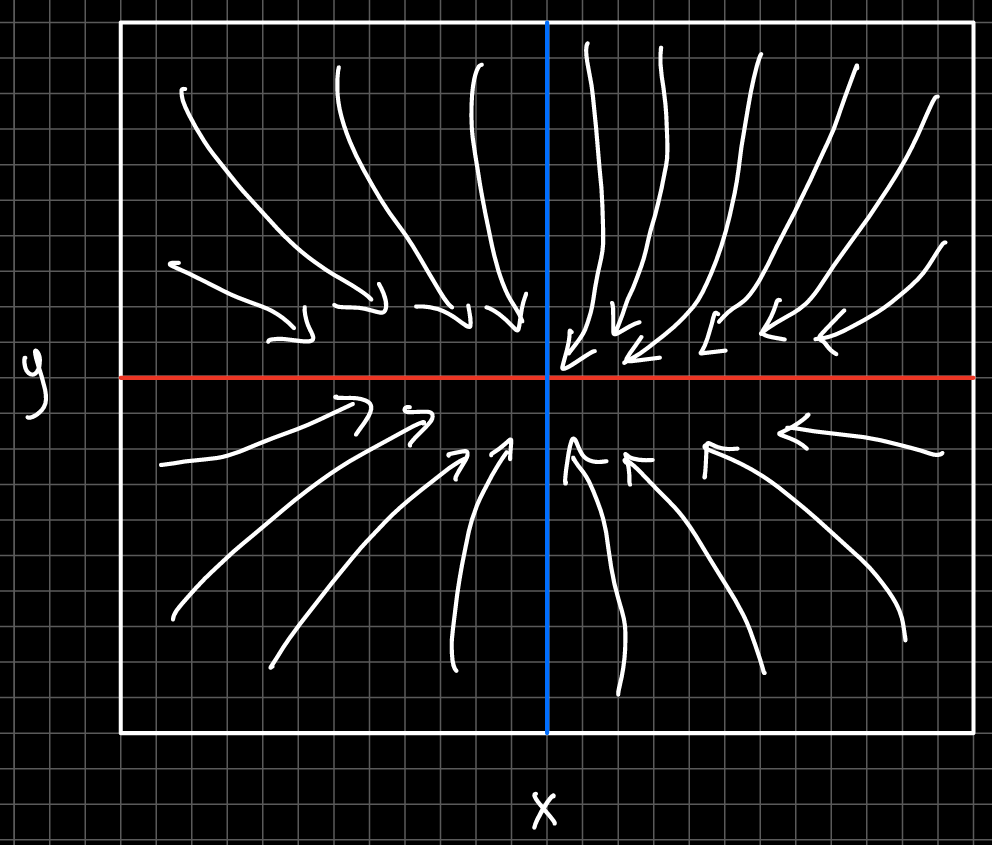
\includegraphics[width=\textwidth]{Screenshot 2026-06-15 193926.png}
        \caption{\(A_N\)}
    \end{subfigure}
    \begin{subfigure}{0.48\textwidth}
        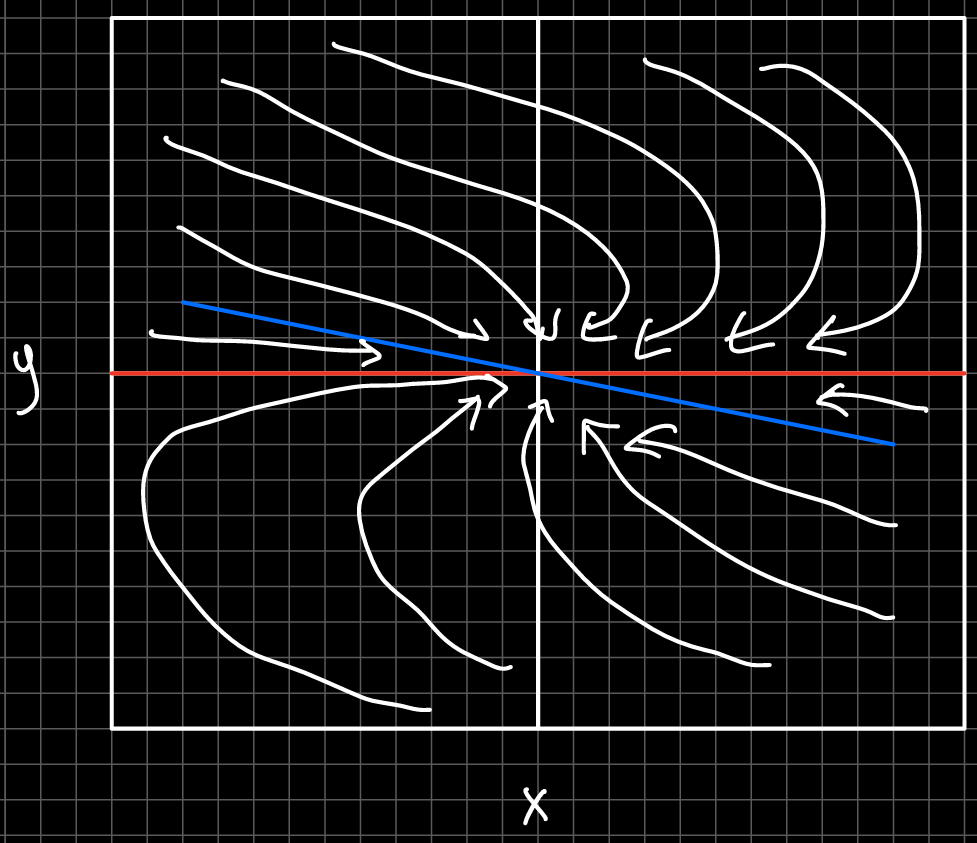
\includegraphics[width=\textwidth]{Screenshot 2026-06-15 193956.png}
        \caption{\(A_{NN}\)}
    \end{subfigure}
\end{figure}
\subsection{Explicit solution }
Since \(A_N\) is diagonal each element is decoupled from the other giving us the solutions
\begin{align}
    x(t) = 0 && y(t)= e^{-2t}
\end{align}
for \(A_{NN}\) we can solve the equation for y immediately and obtain
\begin{equation}
    y(t) = e^{-2t}
\end{equation}
and use this solution for the equation for \(x\)
\begin{equation}
    \dot{x} = -x + 5e^{-2t} \implies x(t) = Ce^{-t}-5e^{-2t}
\end{equation}
inserting \(x(0)=0\) we get \(C=5\) so
\begin{equation}
    x(t) = 5\ins{e^{-t}-e^{-2t}}
\end{equation}
or in other notation
\begin{equation}
    \vb{x}(t) = \ins{5\ins{e^{-t}-e^{-2t}}, e^{-2t}}
\end{equation}
\subsection{growing decaying norm}
Taking the norm of the solution 
\begin{equation}
    N^2 = \norm{\vb{x}(t)}^2 = 25\ins{e^{-t}-e^{-2t}}^2 + e^{-4t}
\end{equation}
redefining parameters to \(u=e^{-t}\)
\begin{equation}
    N^2 = \norm{\vb{x}(t)}^2 = 25\ins{u-u^2}^2+u^4=26u^4-50u^3+25u^2
\end{equation}
plugging into wolfram alpha to find the maximum gives us that there is a local maximum at
\begin{equation}
    t^* \approx 0.648 \quad N \approx \sqrt{1.63}>1
\end{equation}
with no other extrema for \(t>t^*\). But 
\begin{equation}
    N(t=0) = 1
\end{equation}
therefore the norm grows to be larger than the initial value, but then decays.